\documentclass[12pt]{article}
\usepackage[utf8]{inputenc}

\usepackage{amsfonts}
\usepackage{amsmath}
\usepackage{bookmark}
\usepackage[a4paper, margin=3.5cm]{geometry}
\usepackage{graphicx} % For inserting images
\usepackage{hyperref} % For hyperlinks
\usepackage{indentfirst}
\usepackage{minted} % For code-highlighting
\usepackage{parskip}

\graphicspath{ {./images/} }
\setlength{\parindent}{15pt} % Set paragraph indentation
\setlength{\parskip}{1em} % Set paragraph space (one line)
\setminted{frame=single, breaklines} % Set codeblock style

\title{Programming Practicum Report:\\Meeting \#2}
\author{\href{https://github.com/avaxar}{R. Ethan Halim}}
\date{September 2nd, 2024}

\begin{document}

\maketitle

\section{Payslip Calculator}
The entire source file is hosted on a GitHub repository \href{https://github.com/avaxar/uni-practica-1/tree/main/week_2/01_payslip}{\textbf{here}}.

\subsection{Explanation}

\subsubsection{\texttt{Employee} Struct}

In order to encapsulate the properties of an employee's payslip, the said properties are enclosed within a struct: the name as a string, the gross salary, the tax cut, the installment expenditure, the insurance expenditure, and the resulted net salary as unsigned 64-bit integers. In conventional formatting of the Indonesian rupiah, the trailing zeros for the cents (e.g. "\texttt{,00}") are written despite how worthless they are due to historic hyperinflation. However, I shall nevertheless treat them as part of the currency by storing the values in cents directly (hundredths of rupiah) as integers. I refrain from representing them as floating-point numbers, because loss of precision by large values may forfeit monetary integrity.

\begin{minted}{cpp}
struct Employee {
    std::string name;

    // Uses cents instead of rupiah
    uint64_t gross_salary;
    uint64_t tax;
    uint64_t installment;
    uint64_t insurance;
    uint64_t net_salary;
};
\end{minted}

\pagebreak
The struct properties \texttt{name}, \texttt{gross\_salary}, \texttt{installment}, and \texttt{insurance} are user-provided values in the program. The properties \texttt{tax} and \texttt{net\_salary} must therefore be calculated by the program, as per their definitions:
$$\text{Tax} = \text{Gross Salary} \cdot 20\%$$
$$\text{Deductions} = \text{Tax} + \text{Installment} + \text{Insurance}$$
$$\text{Net Salary} = \text{Gross Salary} - \text{Deductions}$$

\subsubsection{\texttt{calculateNet} Function}

In the code, the aforementioned operations and assignments are done by the function \texttt{calculateNet}, which realize the equations above. Its sole argument accepts a reference to an \texttt{Employee} object, where the assignments of \texttt{tax} and \texttt{net\_salary} occur. As it is possible for the deductions to exceed the gross salary, this function also returns a boolean to indicate whether it was successful in calculating the net salary.

\begin{minted}{cpp}
bool calculateNet(Employee& employee) {
    employee.tax = employee.gross_salary / 5; // 20%
    uint64_t deductions = employee.tax + employee.installment + employee.insurance;

    // If the deductions are higher than what the employee has earned
    if (deductions > employee.gross_salary) {
        employee.net_salary = 0;
        return false;
    }
    else {
        employee.net_salary = employee.gross_salary - deductions;
        return true;
    }
}
\end{minted}

\subsubsection{\texttt{formatMoney} Function}

Indonesia uses periods for thousands-separators and commas for decimal points. Therefore, any numbers signifying currency in the printed payslip shall be formatted accordingly, along with the cents. In the code, this utility is implemented by the function \texttt{formatMoney}, which accepts the given currency in cents and returns the formatted string.

\begin{minted}{cpp}
std::string formatMoney(uint64_t cents) {
    ...
}
\end{minted}

There are two important local variables inside of the function: \texttt{original}, which is the string containing the decimal representation of the integer \texttt{cents}; and \texttt{formatted}, which is the string that is to be returned from the function later.

\begin{minted}{cpp}
std::string formatMoney(uint64_t cents) {
    std::string original = std::to_string(cents);
    // The formatted string is constructed backwards.
    std::string formatted = "00,0";

    ...
}
\end{minted}

Note that the formatted string is constructed backwards from the least significant digit to the most significant digit, as hinted by the reversal of the index in the initialization of the \texttt{digit} variable below in the loop. The reason behind so is such that the two digits behind the comma representing the cents can be attended to first in the algorithm following this, before it can then handle with the next subsequent set(s) of three digits, each set of which is to be separated among each other with a thousands-separator (i.e. a period).

\begin{minted}{cpp}
std::string formatMoney(uint64_t cents) {
    ...

    for (size_t i = 0; i < original.length(); i++) {
        char digit = original[original.length() - i - 1];

        // Cents before the comma
        if (i < 2) {
            formatted[i] = digit;
        }
        // First 10^0 digit, replacing '0'
        else if (i == 2) {
            formatted[3] = digit;
        }
        // The rest, where digits must be appended
        else {
            // Add a thousands-separator
            if ((i - 2) % 3 == 0) {
                formatted += '.';
            }

            formatted += digit;
        }
    }

    ...
}
\end{minted}

Finally, upon the conclusion of the formatting, the resulted variable \linebreak \texttt{formatted} is reversed, as to present itself for proper viewing, and is returned with the rupiah currency symbol \texttt{"Rp "} prepended at the front.

\begin{minted}{cpp}
std::string formatMoney(uint64_t cents) {
    ...

    std::reverse(formatted.begin(), formatted.end());
    return "Rp " + formatted;
}
\end{minted}

\subsubsection{\texttt{formatPayslip} Function}

Following the calculation and processing of the input data, which is stored in an \texttt{Employee} struct object, the program is to present it to the terminal. I have made the format to be as follows, where the formatted payslip is given a rectangular border of dashes (\texttt{-}) and vertical bars (\texttt{|}), and there is a one-character margin indenting the text within from both horizontal sides.

\begin{verbatim}
 -----------------------------------
| Payslip for Employee              |
|-----------------------------------|
| Name         : [Name of Employee] |
| Gross Salary : [Gross Salary]     |
| Tax (20%)    : [Tax Cut]          |
| Installment  : [Installment]      |
| Insurance    : [Insurance]        |
| Net Salary   : [Net Salary]       |
 -----------------------------------
\end{verbatim}

In the code, this utility is implemented by the function \texttt{formatPayslip}, which accepts the provided \texttt{Employee} struct object whose properties shall be displayed. As the data within will only be read and not written to, a const-reference is used for the argument, as to not entirely duplicate the content.

\begin{minted}{cpp}
std::string formatPayslip(const Employee& employee) {
    ...
}
\end{minted}

Each line in the content of the report is put inside of a vector, where the label of each property is prepended directly. As for the monetary properties, it can be seen below that the previous \texttt{formatMoney} function is utilized for currency-formatting. Additionally, in order to be able to calculate the number of preceding spaces for each line as to align the right border properly, the STL function \texttt{std::max\_element} is used with a lambda to compare for the line string with the largest length in further comparison with the report title.

\begin{minted}{cpp}
std::string formatPayslip(const Employee& employee) {
    std::string title = "Payslip for Employee";
    std::vector<std::string> lines = // Payslip information
        {"Name         : " + employee.name,
         "Gross Salary : " + formatMoney(employee.gross_salary),
         "Tax (20%)    : " + formatMoney(employee.tax),
         "Installment  : " + formatMoney(employee.installment),
         "Insurance    : " + formatMoney(employee.insurance),
         "Net Salary   : " + formatMoney(employee.net_salary)};

    // Figures out the maximum amount of characters needed in width
    size_t max_width =
        std::max_element(lines.begin(), lines.end(), [](std::string& a, std::string& b) {
            return a.length() < b.length();
        })->length();
    max_width = std::max(max_width, title.length());

    ...
}
\end{minted}

As for the generation of the formatted report itself, each line is appended to the resulted variable that shall be passed as the return value --- \texttt{formatted}. For performance optimization, I made use of the \texttt{.reserve} method provided in \texttt{std::string}, in order to provide the expected amount of characters that will be filled in the string, taking into factor the character width, height, and border margins, in order to minimize memory reallocations. The function generates the top border out of dashes, the title with side borders with vertical bars, the title-content separator out of dashes, the lines themselves with the proper amount of aligning spaces, as well as the bottom border out of dashes.

\begin{minted}{cpp}
std::string formatPayslip(const Employee& employee) {
    ...

    std::string formatted;
    // Reserves the appropriate amount of characters that will be fit, as to prevent reallocation for expansion in the heap
    formatted.reserve((max_width + 5) * (lines.size() + 4) + 1);

    formatted += " -" + std::string(max_width, '-') + "- \n";                          // Top border
    formatted += "| " + title + std::string(max_width - title.length(), ' ') + " |\n"; // Title
    formatted += "|-" + std::string(max_width, '-') + "-|\n";                          // Separator

    for (const std::string& line : lines) {
        formatted += "| " + line + std::string(max_width - line.length(), ' ') + " |\n";
    }

    formatted += " -" + std::string(max_width, '-') + "- \n"; // Bottom border

    return formatted;
}
\end{minted}

\subsubsection{Main Program}

Below is the main program itself, enclosed within the function \texttt{program} whose arguments provide references to the input and output streams. The program receives input from the user, requesting the employee's name, gross salary, installment expenditure, and insurance expenditure. Utilizing the previous \texttt{calculateNet} function, the \texttt{Employee} struct object (initialized as the \texttt{employee} variable) is calculated of its tax and net salary. The payslip is then generated by the \texttt{formatPayslip} function and printed out.

\begin{minted}{cpp}
int program(std::istream& cin, std::ostream& cout) {
    Employee employee;

    cout << "Insert name: ";
    std::getline(cin, employee.name);

    cout << "Insert gross salary: ";
    cin >> employee.gross_salary;
    employee.gross_salary *= 100; // Rupiah to cents

    cout << "Insert installment: ";
    cin >> employee.installment;
    employee.installment *= 100; // Rupiah to cents

    cout << "Insert insurance cost: ";
    cin >> employee.insurance;
    employee.insurance *= 100; // Rupiah to cents

    if (!calculateNet(employee)) {
        cout << "The deductions are higher than the gross salary!\n";
        return 1;
    }

    cout << '\n' << formatPayslip(employee);

    return 0;
}
\end{minted}

As implemented before, the function \texttt{calculateNet} is made to return \texttt{false} if it fails to calculate the proper net salary of the employee due to the deductions exceeding the gross salary. Upon such case, the main program warns the user of the issue and exits the program with an error code.

\begin{minted}{cpp}
int program(std::istream& cin, std::ostream& cout) {
    ...

    if (!calculateNet(employee)) {
        cout << "The deductions are higher than the gross salary!\n";
        return 1;
    }

    ...
}
\end{minted}

\subsection{Manual Testing}
Below is the compilation and the testing of the source code. As can be seen, the program successfully calculated the tax and net salary, and formatted the stylized payslip correctly.
\newline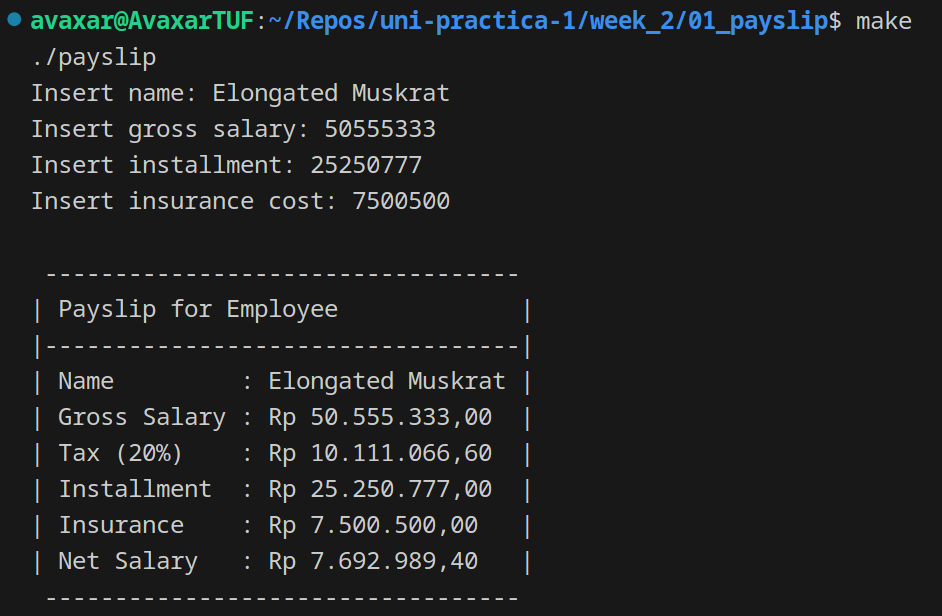
\includegraphics[width=\textwidth]{01_payslip}

\subsection{Test Cases}

\subsubsection{Tests}
Below is copied directly from the \texttt{tests.txt} file.
\inputminted{text}{01_payslip/tests.txt}

\subsubsection{Execution}
Below are the results of the test cases. No test cases failed.
\newline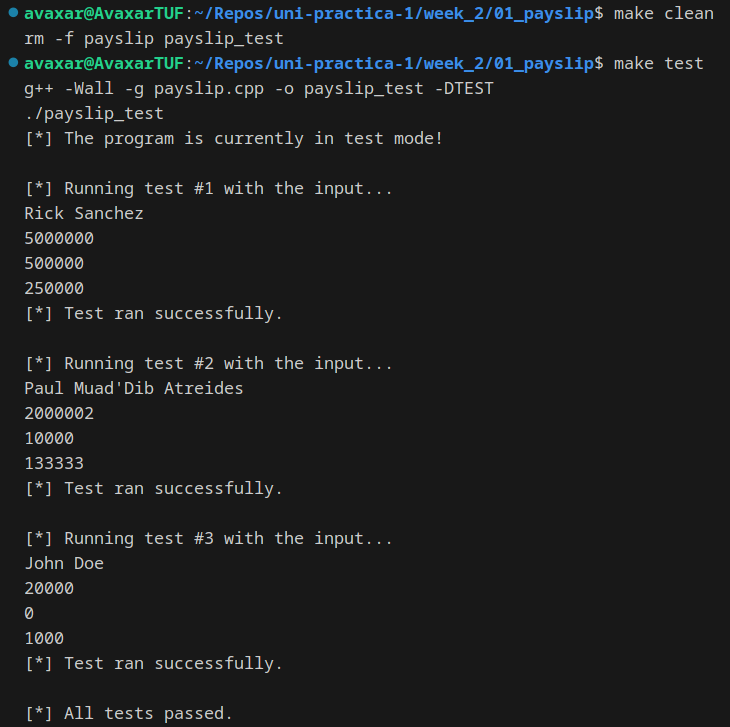
\includegraphics[width=\textwidth]{01_payslip_test}

\pagebreak
\section{Quadratic Equation Solver}
The entire source file is hosted on a GitHub repository \href{https://github.com/avaxar/uni-practica-1/tree/main/week_2/02_quadratic}{\textbf{here}}.

\subsection{Explanation}

\subsubsection{\texttt{RootType} Enum}

In order to represent states, any of which can be the type of the result of the quadratic formula (i.e. having two distinct roots, having one single root, or having complex roots), I implemented the \texttt{RootType} enum type to represent the said state enumerations.

\begin{minted}{cpp}
enum class RootType {
    DISTINCT,
    SINGLE,
    COMPLEX
};
\end{minted}

\subsubsection{\texttt{quadratic} Function}

$$ax^2 + bx + c = 0$$
$$\text{discriminant} = D \equiv b^2 - 4ac$$
$$x = \frac{-b \pm \sqrt{D}}{2a}$$

The \texttt{quadratic} function directly implements the quadratic formula as defined above, which finds the roots of a quadratic equation, given the three coefficients. However, the function also needs to inform whether the root(s) are in one of the three states: being two distinct real values, being one single real value, or being complex values. Therefore, the discriminant of the equation is calculated, in order to determine the said state, which is represented as a \texttt{RootType} enumeration. The enumeration shall be returned from the function for handling by the main program, and the potential roots shall be assigned to the \texttt{x1} and \texttt{x2} reference arguments.

\begin{minted}{cpp}
RootType quadratic(double a, double b, double c, double& x1, double& x2) {
    double discriminant = std::pow(b, 2.0) - 4.0 * a * c;

    // There are two distinct real roots.
    if (discriminant > 0.0) {
        x1 = (-b + std::sqrt(discriminant)) / (2.0 * a);
        x2 = (-b - std::sqrt(discriminant)) / (2.0 * a);

        return RootType::DISTINCT;
    }
    // There is only one single real root.
    else if (discriminant == 0.0) {
        // Assigns both output arguments with the same value
        x1 = x2 = -b / (2.0 * a);

        return RootType::SINGLE;
    }
    // The roots are non-real/complex.
    else {
        // Sets both output arguments to NaN
        x1 = x2 = NAN;

        return RootType::COMPLEX;
    }
}
\end{minted}

\subsubsection{Main Program}
Below is the main program itself, enclosed within the function program whose arguments provide references to the input and output streams. The program receives input from the user, requesting the $a$, $b$, and $c$ coefficients for the quadratic equation to be solved.

\begin{minted}{cpp}
int program(std::istream& cin, std::ostream& cout) {
    double a, b, c;
    cout << "Insert `a`: ";
    cin >> a;
    cout << "Insert `b`: ";
    cin >> b;
    cout << "Insert `c`: ";
    cin >> c;

    ...
}
\end{minted}

The program utilizes a switch-statement to handle the possible enumerated states from the \texttt{quadratic} function. It prints to the terminal and informs the user of whether the resulted root(s) are distinct, single, or complex, as well as gives the value(s) if they are real value(s).

\begin{minted}{cpp}
int program(std::istream& cin, std::ostream& cout) {
    ...

    double x1, x2;
    switch (quadratic(a, b, c, x1, x2)) {
        case RootType::DISTINCT:
            cout << "\nThere are two distinct real roots: " << x1 << " and " << x2 << ".\n";
            break;

        case RootType::SINGLE:
            cout << "\nThere is only one single real root: " << x1 << ".\n";
            break;

        case RootType::COMPLEX:
            cout << "\nThere are no real roots; the roots are complex.\n";
            break;
    }

    return 0;
}
\end{minted}

\subsection{Manual Testing}
Below is the compilation and the testing of the source code.
\newline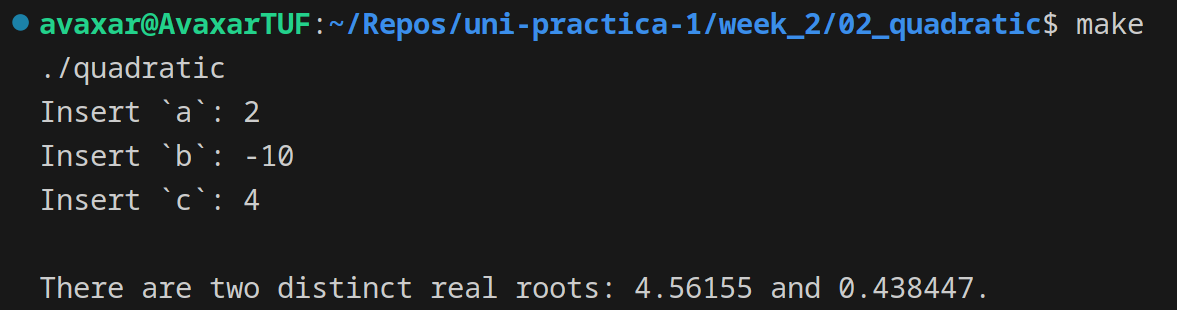
\includegraphics[width=\textwidth]{02_quadratic}

\subsection{Test Cases}

\subsubsection{Tests}
Below is copied directly from the \texttt{tests.txt} file. The first two test cases test for the scenario where there are two distinct real roots; the second two test cases test for the scenario where there is only one single real root; and the third two test cases test for the scenario where the roots are complex.
\inputminted{text}{02_quadratic/tests.txt}

\subsubsection{Execution}
Below are the results of the test cases. No test cases failed.
\newline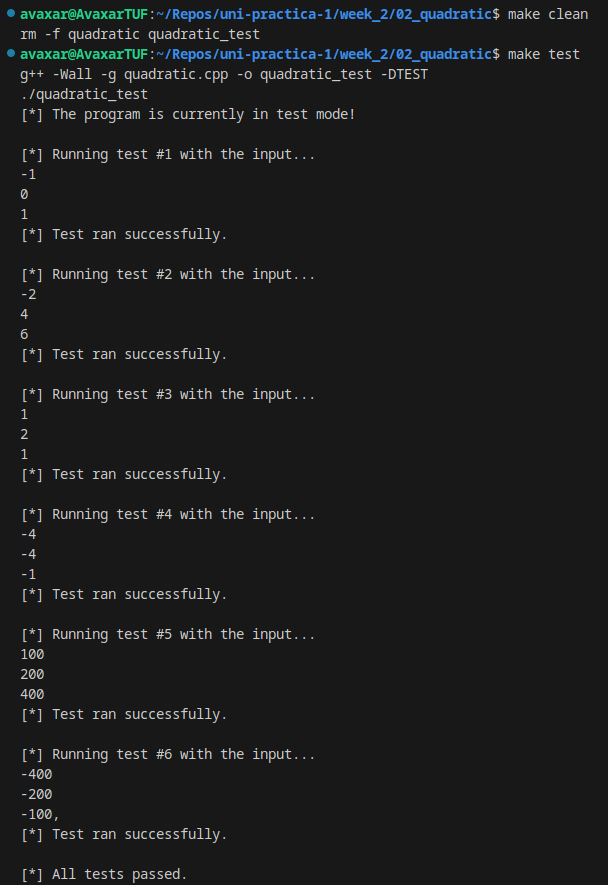
\includegraphics[width=\textwidth]{02_quadratic_test}

\end{document}
